\documentclass[12pt,notheorems,hyperref={pdfauthor=Professor Rafael Nardi}]{beamer}

% Copyright (c) 2022 by Lars Spreng
% This work is licensed under the Creative Commons Attribution 4.0 International License. 
% To view a copy of this license, visit http://creativecommons.org/licenses/by/4.0/ or send a letter to Creative Commons, PO Box 1866, Mountain View, CA 94042, USA.

%~~~~~~~~~~~~~~~~~~~~~~~~~~~~~~~~~~~~~~~~~~~~~~~~~~~~~~~~~~~~~~~~~~~~~~~~~~~~~~
% Add your packages and commands to this file
%~~~~~~~~~~~~~~~~~~~~~~~~~~~~~~~~~~~~~~~~~~~~~~~~~~~~~~~~~~~~~~~~~~~~~~~~~~~~~~

%~~~~~~~~~~~~~~~~~~~~~~~~~~~~~~~~~~~~~~~~~~~~~~~~~~~~~~~~~~~~~~~~~~~~~~~~~~~~~~
\RequirePackage{palatino}
\RequirePackage[utf8]{inputenc}
\RequirePackage[T1]{fontenc}

\usefonttheme{serif}

\usepackage{styles/elegantmacros}
\usefolder{styles}
\usetheme[style=blue]{elegant}

\newcommand{\makepart}[1]{ % For convenience
\part{#1} \frame{\partpage}
}

%~~~~~~~~~~~~~~~~~~~~~~~~~~~~~~~~~~~~~~~~~~~~~~~~~~~~~~~~~~~~~~~~~~~~~~~~~~~~~~

%~~~~~~~~~~~~~~~~~~~~~~~~~~~~~~~~~~~~~~~~~~~~~~~~~~~~~~~~~~~~~~~~~~~~~~~~~~~~~~
% Figures
\RequirePackage{booktabs}
\RequirePackage{colortbl}
\RequirePackage{ragged2e}
\RequirePackage{schemabloc}
%\RequirePackage{natbib}
\RequirePackage{caption}
\RequirePackage{subcaption}
\RequirePackage{tabularx}
\RequirePackage{array}
\RequirePackage{multirow}
\usepackage[
  style=authoryear, 
]{biblatex}
\addbibresource{references.bib}
\newcolumntype{Y}{>{\centering\arraybackslash}X}

%~~~~~~~~~~~~~~~~~~~~~~~~~~~~~~~~~~~~~~~~~~~~~~~~~~~~~~~~~~~~~~~~~~~~~~~~~~~~~~

%~~~~~~~~~~~~~~~~~~~~~~~~~~~~~~~~~~~~~~~~~~~~~~~~~~~~~~~~~~~~~~~~~~~~~~~~~~~~~~
% Figures
\RequirePackage{wrapfig}
\RequirePackage{pgfplots}
\RequirePackage{graphicx}
\RequirePackage{adjustbox}
\RequirePackage{environ}
\pgfplotsset{compat=1.18}

\makeatletter
\newsavebox{\measure@tikzpicture}
\NewEnviron{scaletikzpicturetowidth}[1]{%
  \def\tikz@width{#1}%
  \def\tikzscale{1}\begin{lrbox}{\measure@tikzpicture}%
  \BODY
  \end{lrbox}%
  \pgfmathparse{#1/\wd\measure@tikzpicture}%
  \edef\tikzscale{\pgfmathresult}%
  \BODY
}
\makeatother
%~~~~~~~~~~~~~~~~~~~~~~~~~~~~~~~~~~~~~~~~~~~~~~~~~~~~~~~~~~~~~~~~~~~~~~~~~~~~~~

%~~~~~~~~~~~~~~~~~~~~~~~~~~~~~~~~~~~~~~~~~~~~~~~~~~~~~~~~~~~~~~~~~~~~~~~~~~~~~~
% Maths 
\RequirePackage{textcomp}
\RequirePackage{amsmath} 
\RequirePackage{amsthm}
\RequirePackage{mathtools}
%\RequirePackage{bbm}
%\RequirePackage{algorithm}
%\RequirePackage[osf,sc]{mathpazo}
%\RequirePackage{pifont}
%\newcommand{\xmark}{\ding{55}}%
%\numberwithin{equation}{section}
\DeclareMathOperator*{\argmax}{arg\,max}
\DeclareMathOperator*{\argmin}{arg\,min}

\setbeamertemplate{theorems}[numbered] % to number

\theoremstyle{definition}
\newtheorem{fact}{Fact}[section]
\newtheorem{examp}{Example}[section]

\theoremstyle{plain}
\newtheorem{definition}{Definition}[section]
\newtheorem{proposition}{Proposition}
\newtheorem{theorem}{Theorem}
\newtheorem{assumption}{Assumption}

\providecommand{\H}{\mathscr{H}}      
\providecommand{\E}{\mathbb{E}}
\makeatletter
\def\munderbar#1{\underline{\sbox\tw@{$#1$}\dp\tw@\z@\box\tw@}}
\makeatother

%~~~~~~~~~~~~~~~~~~~~~~~~~~~~~~~~~~~~~~~~~~~~~~~~~~~~~~~~~~~~~~~~~~~~~~~~~~~~~~



% \usepackage{subfigure}

\title{Energia Solar Térmica}
\subtitle{Modelo de Torre Central}
\author{Professor Rafael Nardi}
\institute{UFSB}
\date{Janeiro/2023}



\begin{document}

{
\setbeamertemplate{footline}{} 
\begin{frame}%Capa
  \titlepage
	\begin{figure}[b]
		\centering
		
\includegraphics[scale=0.5]{./logo_ufsb.png}
	\end{figure}
\end{frame}
}

\addtocounter{framenumber}{-1}

\section{Tecnologias CSP e Fotovoltaica}

\begin{frame}%Sol: fonte primária

	Com exceção da energia nuclear e das marés, indiretamente, o sol é a fonte de todas
	fontes de energia usadas pela humanidade. \pause

	\bigskip

	\begin{itemize}
			\item Uso indireto: biomassa, eólica, hidroelétrica.
	\end{itemize} \pause

	\bigskip

	\begin{itemize}
		\item Duas formas de uso direto :
			\medskip
		\begin{itemize}
			\item Fotovoltaica: conversão direta da radiação em corrente elétrica \pause
			\medskip
			\item CSP (Concentrated Solar Power): radiação é concentrada e calor é usado para tocar uma máquina térmica
		\end{itemize}

	\end{itemize}

\end{frame}

\subsection{Plantas Fotovoltaicas}

\begin{frame}%Desert Tenger China - Fotovolt

	\begin{itemize}
		\item Parque Solar Desert Tenger, China. $1200$ $km^2$. Potência de $1$ GW na fase inicial e $3$
			GW em operação plena. (Maior do Mundo) \footnote{ \href{https://www.globaltimes.cn/page/202209/1275050.shtml}{Fonte: Gobal Times}}
	\end{itemize}

	\begin{figure}
		\centering
		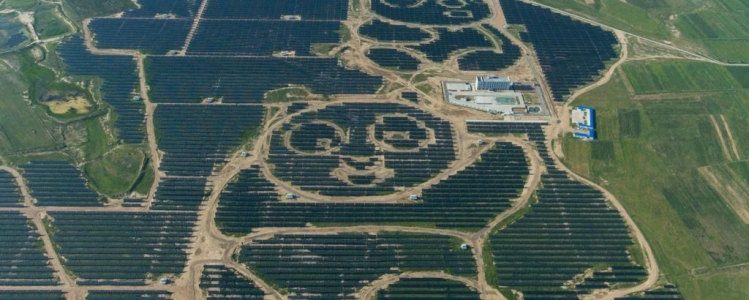
\includegraphics[scale=0.45]{./92336_parquesolardeserttenger.jpg}
	\end{figure}

\end{frame}

\begin{frame}%Piauí

	\begin{itemize}
		\item Parque Solar São Gonçalo, Piauí. $2$ milhões de painéis. $12$ milhões de
	$m^2$ ($1500$ estádios de futebol). Potência atual de $575,725$ MW que será
	extendida a $864$ MW. (Maior da américa latina.) \footnote{ \href{https://www.enelgreenpower.com/pt/nossos-projetos/highlights/parque-solar-sao-goncalo}{Fonte: Enel Green Power}}
	\end{itemize}

	\begin{figure}
		\centering
		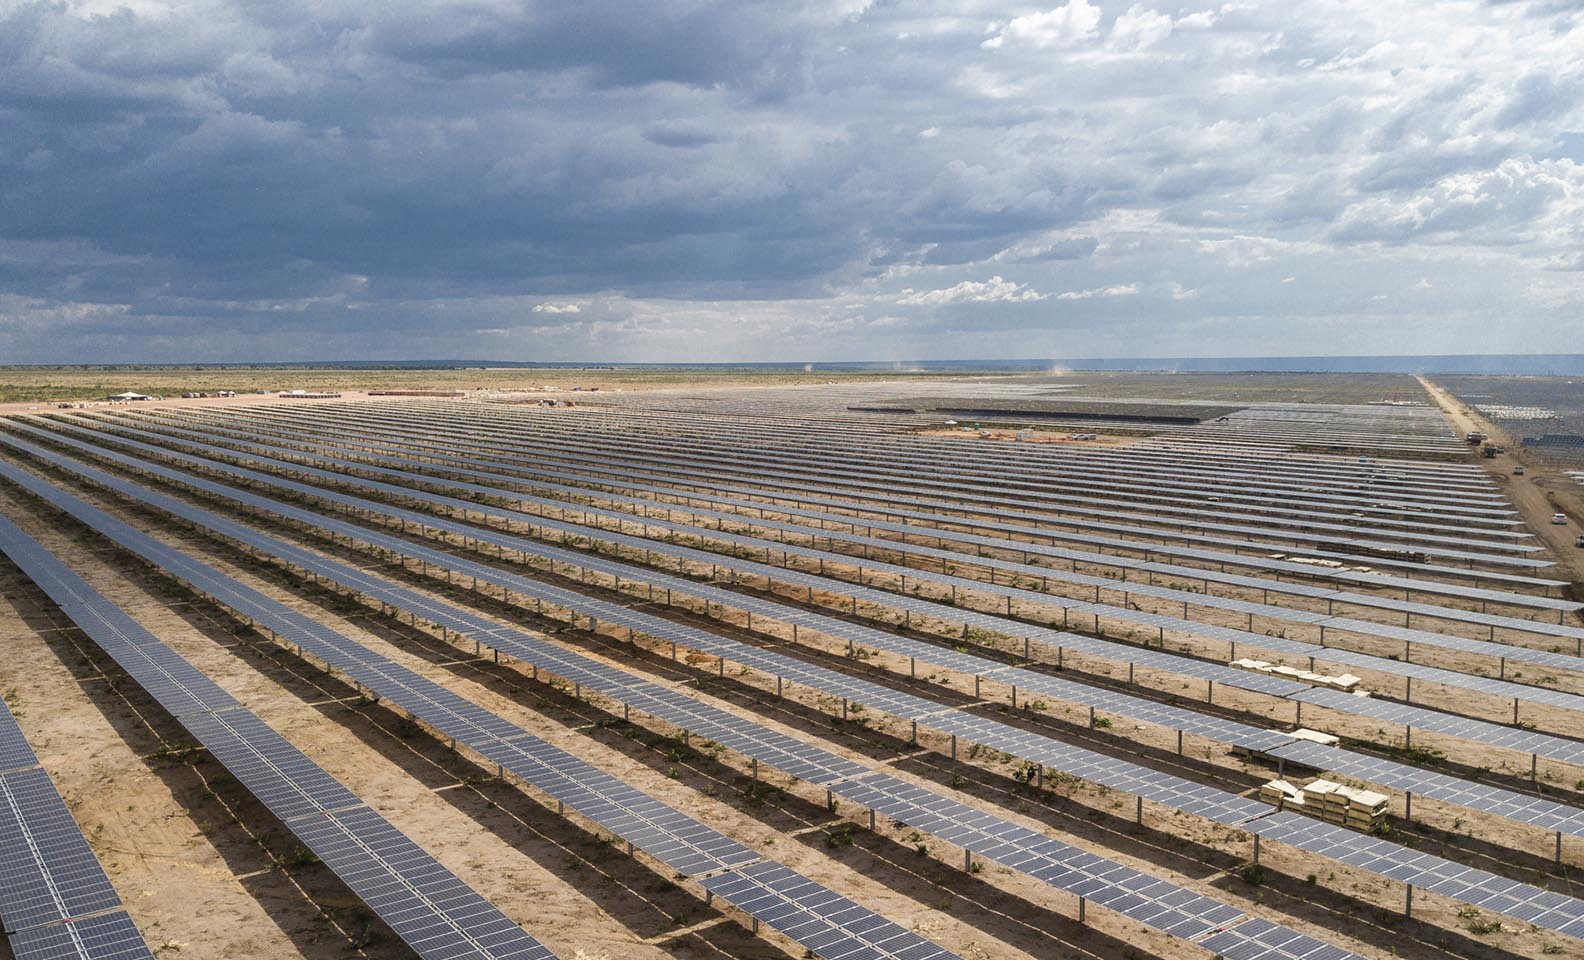
\includegraphics[scale=0.38]{./parco-solare-sao-goncalo_1584x960.jpg}
	\end{figure}

\end{frame}

\subsection{Plantas CSP - Torre Central}


\begin{frame}%Ivanpah - Torre central

	\begin{itemize} \item Projeto Ivanpah, California. Em operação desde 2014.
		Potência de $392$ MW. $940$ mil MW/h por ano de energia produzida. $1,6$
		bilhões de dólares investidos. $173500$ Heliostatos.
\footnote{ \href{https://www.energy.gov/lpo/ivanpah}{Fonte: Departamento de energia dos EUA}} \end{itemize}

	\begin{figure}
		\centering
		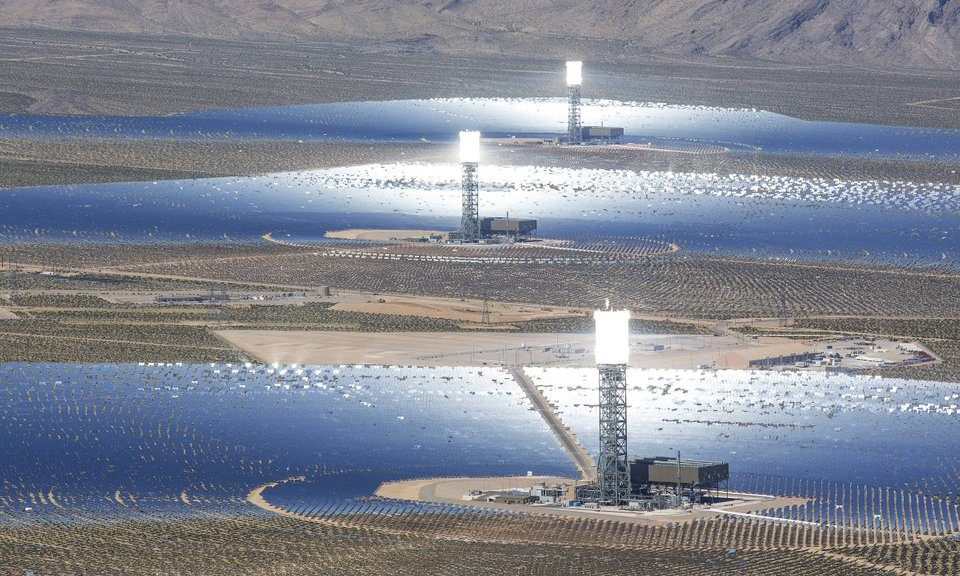
\includegraphics[scale=0.3]{./Ivanpah4-960x576.jpg}
	\end{figure}

\end{frame}

\begin{frame}%Espanha 

	\begin{itemize} 
		\item PS10 (Não é o play station!) nas proximidades de Sevilha/Espanha. Em operação desde 2007.
			Capacidade de produção em $11$ MW e parte de um projeto com
			$300$ MW de capacidade. São $640$ heliostatos de $120$ $m^2$ de área e uma torre central de $115$ m de altura.
			Custo de $1,2$ bilhões de euros (para os $300$ MW). \footnote{\href{https://www.power-technology.com/projects/seville-solar-tower/}{Fonte: power-technology.com}}
	\end{itemize}

	\begin{figure}
		\centering
		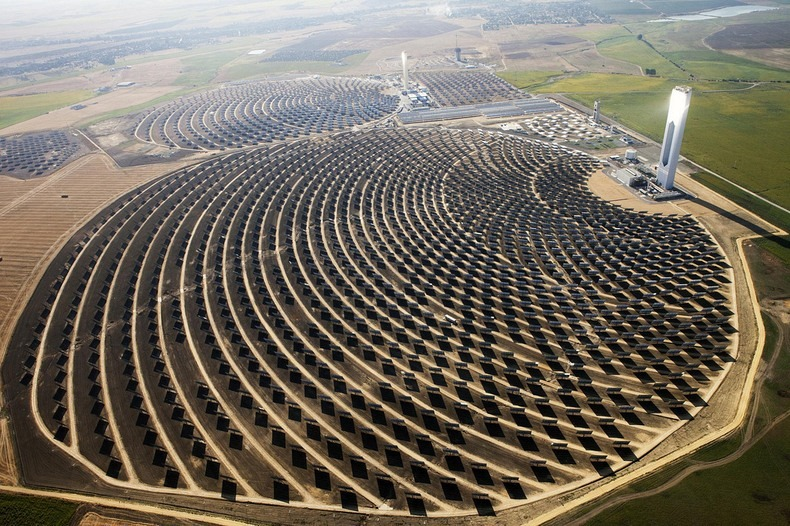
\includegraphics[scale=0.3]{./seville-solar-plant-10[6].jpg}
	\end{figure}

\end{frame}

\subsection{Plantas CSP - Calha Parabólica}

\begin{frame}%Shams 1 - Emirados Árabes Unidos

	\begin{itemize} 
		\item Localizado nos Emirados Árabes Unidos, iniciou o funcionamento em
			2013. Capacidade nominal de $100$ MW. Cobre uma área de $2,5$
			$\text{km}^2$. Investimento de $648$ milhões de dólares produzindo
			energia a um custo médio nivelado de $0,27$ USD/kW. Área de coletores:
			$627840$ $\text{m}^2$.  \footnote{\href{portal petronoticias.com.br}{Fonte: National Renewable Energy Laboratory/USA}}
	\end{itemize}

	\bigskip

	\begin{figure}[ht]
		\centering
		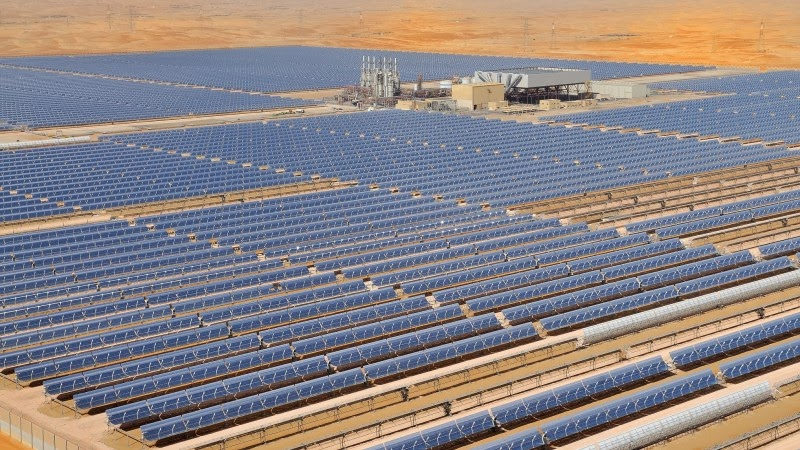
\includegraphics[scale=0.35]{./Shams_1.jpg}
	\end{figure}

\end{frame}

\begin{frame}%Calha parabólica - São Paulo

	\begin{itemize} 
		\item Projeto da CESP em Rosana/SP inaugurado em março de 2022. Capacidade
			de $0,5$ MW. Investimento de $57$ milhões de reais em desenvolvimento desde 2017. \footnote{\href{https://petronoticias.com.br/cesp-inaugurou-a-primeira-usina-termossolar-do-pais-em-sao-paulo/}{Fonte: portal petronoticias.com.br}}
	\end{itemize}

	\bigskip

	\begin{figure}[ht]

		\begin{minipage}[b]{.4\linewidth}
			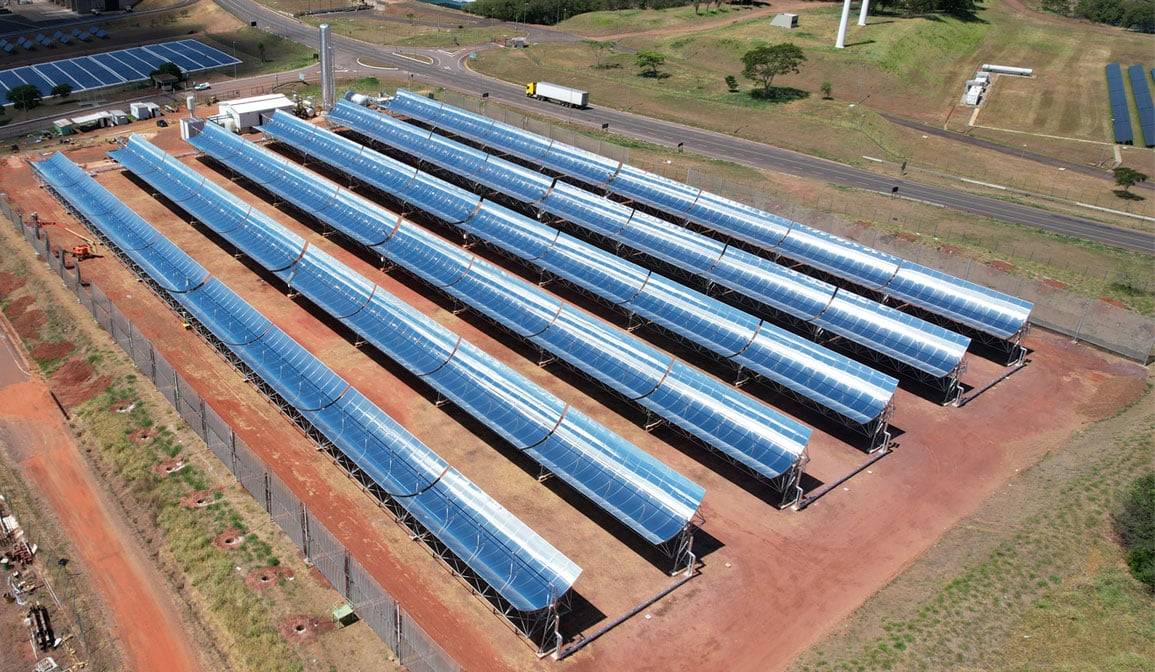
\includegraphics[height=0.62\linewidth]{./CESP_Rosana-SP.jpg}
		\end{minipage}
		\qquad
		\begin{minipage}[b]{.4\linewidth}
			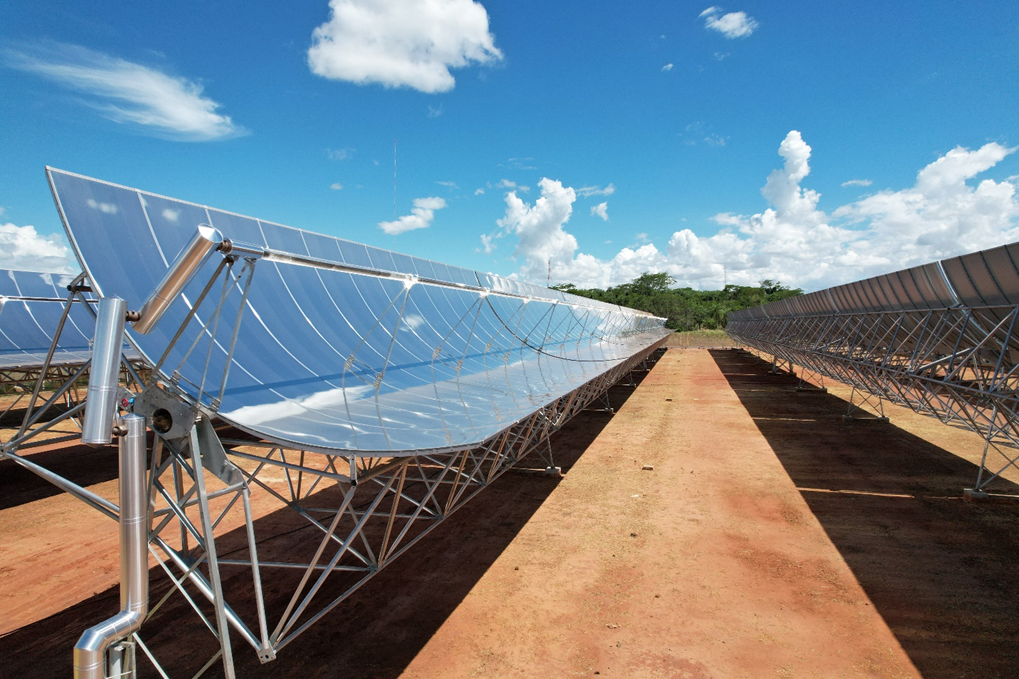
\includegraphics[height=0.62\linewidth]{./CESP_Rosana-SP_2.png}
		\end{minipage}
	\end{figure}

\end{frame}

\subsection{Plantas CSP - Pratos Parabólicos}

\begin{frame}%

	\begin{itemize} 
		\item Maricopa Power Plant, Arizona/EUA iniciado em 2010. 60 discos
			parabólicos, cada um gerando $25$ kW de potência nominal através de um
			motor Stirling posicionado no foco do disco totalizando $1,5$ MW. \footnote{\href{https://www.powermag.com/dish-stirling-solar-plant-debuts/}{Fonte: portal Powermag.com}} Empresa
			faliu em 2012 e o projeto foi descontinuado. \footnote{\href{https://www.bizjournals.com/phoenix/news/2012/03/27/former-stirling-power-plant-in-peoria.html}{Fonte: Phoenix Business Journal}}
			
	\end{itemize}

	\bigskip

	\begin{figure}[ht]
		\centering
		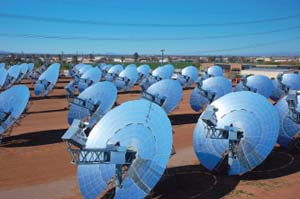
\includegraphics[scale=0.65]{./parab_dishes_1.jpeg}
	\end{figure}

\end{frame}

\subsection{Fotovoltaica e CSP - Comparativo}

\begin{frame}%Potência instalada Mundo

	\begin{table}
		\begin{tabular}{lc}
			\toprule
			Tecnologia & Potência instalada (Mundo) \footnote{ \href{https://www.iee.usp.br/}{Fonte: IEE-USP}}\\
			\midrule
			Fotovoltaica &  456 GW \\
			CSP &  6 GW  \\
			\bottomrule
		\end{tabular}
	\end{table}

\end{frame}

\begin{frame}%Potência instalada Brasil

	\begin{table}
		\begin{tabular}{lc}
			\toprule
			Tecnologia & Potência instalada (Brasil) \footnote{\href{https://www.iee.usp.br/}{Fonte: IEE-USP}}\\
			\midrule
			Fotovoltaica & 4 GW  \\
			CSP &  100 MG  \\
			\bottomrule
		\end{tabular}		
		
	\end{table}
	
\end{frame}

\begin{frame}%Eficiência

	\begin{table} 
		\begin{tabular}{lc}
			\toprule
			Tecnologia & Eficiência  \footnote{\href{https://resources.solarbusinesshub.com/solar-industry-reports/item/renewable-power-generation-costs-in-2019}{Fonte: Renewable Power Generation Costs in 2019, IRENA}}\\
			\midrule
			Fotovoltaica & 15-20\% \\
			CSP & 20-30\% \\
			\bottomrule
		\end{tabular}
	\end{table}
	
\end{frame}

\begin{frame}%custos

	\begin{table}
		\begin{tabular}{lc}
			\toprule
			Tecnologia & Custo \footnote{\href{https://resources.solarbusinesshub.com/solar-industry-reports/item/renewable-power-generation-costs-in-2019}{Fonte: Renewable Power Generation Costs in 2019, IRENA}}\\
			\midrule
			Fotovoltaica & 0,10 - 0,30 US\$ \\
			CSP & 0,15 - 0,20 US\$ \\
			\bottomrule
		\end{tabular}
	\end{table}
	
\end{frame}

\section{Modelo de Torre Central}

\subsection{Características gerais}

\begin{frame}
	\begin{itemize}
		\item Princípio de funcionamento: uma malha de espelhos (heliostatos)
			refletem a luz do sol num único ponto focal. O calor produzido é
			convertido em movimento de uma turbina (ciclo Rankine ou Brayton) que
			conectada a um gerador, produz eletricidade.\pause
		\item altas temperaturas atingidas elevam a eficiência.\pause
		\item sal fundido tem sido usado como fluido para a troca de calor na
			torre. (alta capacidade térmica do sal) \pause
		\item indicado para produção de energia em grande escala.\pause
		\item latitudes mais indicadas: entre $15^o$ a $40^o$. Ilhéus: $14,79^o$.\pause
		\item principal vantagem das tecnolgias CSP em relação à fotovoltaica é a
			capacidade de armazenar energia na forma de calor para conversão em
			eletricidade em picos de demanda.\pause
		\item Baixo impacto ambiental: pouca demanda de espaço, água e pouco impacto visual.\pause
		\item torres centrais correspondem a $15\%$ das plantas operacionais e são
			a segunda tecnologia mais madura, atrás das calhas parabólicas com
			$80\%$ das plantas operacionais.
	\end{itemize}
\end{frame}

\subsection{Parâmetros envolvidos na produção de energia}

\begin{frame}%Todos parâmetros
	\begin{itemize}
		\item Qualidade do recurso solar (percentual de radiação direta em relação à difusa)
			\begin{itemize}
				\item Latitude
				\item Altitude
				\item Vapor de água
				\item Poeira em suspensão
				\item Aerosol
				\item Absorção por ar seco
			\end{itemize} \pause
			\bigskip
		\item Geometria do campo de heliostatos
			\begin{itemize}
				\item Quantidade e disposição dos heliostatos
				\item Altura da torre central
				\item Hora do dia e período do ano
			\end{itemize} \pause
			\bigskip
		\item Ciclo termodinâmico de conversão de calor em eletricidade
			\begin{itemize}
				\item Temperatura no ponto focal
				\item Tipo de fluido
			\end{itemize}
	\end{itemize}
\end{frame}

\begin{frame}%Iqbal e caminho optico na atmosfera
	Para modelagem de absorção atmosférica usamos a teoria exposta no livro ``\emph{An
	Introduction to solar radiation}'', M. Iqbal (1983).
\begin{figure}[htpb]
		\centering
			\begin{tikzpicture}[scale=0.7, transform shape]
				\def\squareSize{4}
				\tkzInit[xmin=-\squareSize,xmax=+\squareSize,ymin=-\squareSize,ymax=\squareSize]
				\tkzDefPoint(0,0){O}
				\tkzDefPoint(0,2.5){A}
				\tkzDefPoint(0,4){B}
				\tkzDefPoint(55:4){C} \tkzDefPoint(55:0.7){c}
				\tkzDefPoint(55:2.5){E}
				\tkzDrawCircle(O,A)
				\tkzDrawCircle(O,B)
				\tkzDrawSegment[dashed](O,B)
				\tkzDrawSegment[dashed](O,C)
				\tkzDrawSegment[red](A,C)
				\tkzDefPointBy[projection=onto O--B](C) \tkzGetPoint{D}
				\tkzDrawSegment[dashed](D,C)

				\tkzDefMidPoint(O,E) \tkzGetPoint{Rt} \tkzLabelPoint[below right](Rt){$R_T$}
				\tkzDefMidPoint(E,C) \tkzGetPoint{H} \tkzLabelPoint[below right](H){$H$}
				\tkzDefMidPoint(A,D) \tkzGetPoint{h} \tkzLabelPoint[left](h){$h$}
				\tkzDefMidPoint(C,D) \tkzGetPoint{l} \tkzLabelPoint[above](l){$l$}
				\tkzDefMidPoint(A,C) \tkzGetPoint{d} \tkzLabelPoint[below, red](d){$d$}

				\tkzDrawArc[black](O,c)(A) \tkzLabelPoint[above]({70.5:0.7}){$\alpha$}

				\tkzDefPointWith[linear, K=0.15](A,C) \tkzGetPoint{zen_angle}
				\tkzDrawArc[black](A,zen_angle)(B) 

				\tkzDefPointBy[rotation=center A angle 20](zen_angle) 
				\tkzLabelPoint[above](tkzPointResult){$\theta_z$}

				\tkzLabelPoint(65:5.2){$d \sim \frac{1}{\cos(\theta_z)}$}
			\end{tikzpicture}
		
			\caption{{\color{red} Caminho} do raio de luz na atmosfera.}%
		\label{fig:caminho_luz_na_atmosfera}
	\end{figure}

\end{frame}

\begin{frame}%Gráfico - dependência com altitude

	\begin{figure}[htpb]
		\centering
		\centering 
		\begin{tikzpicture}[scale=0.5]
			\node[draw, align=left] at (-6,7) {\scriptsize Latitude: $-18,9$ \\ \scriptsize Dia do ano: 16/03 \\ \scriptsize Hora local: $12h$ \\ \scriptsize Umidade relativa: $80\%$ \\ \scriptsize Parâmetro de poeira: $200$};
			\begin{axis}[
				height=16cm, 
				width=16cm, 
				grid=both, 
				grid style={line width=.1pt, draw=gray!20},
				major grid style={line width=.2pt,draw=gray!50}, 
				minor tick num=4, 
				xlabel={Altitude}, 
				ylabel={Percentual}, 
				title={Variação da potência que chega ao solo com a altitude.}
				]
				\addplot[mark size=0.5pt, color=blue] table[x=altitude, y=PercentTransm, col sep=semicolon] {../../../data/aten_corr_data/corrected_J_dep_on_altitude.dat};
			\end{axis}
		\end{tikzpicture}
		% \caption{Variação da potência que chega ao solo com a altitude.} 
		\label{fig:altitude}
	\end{figure}
\end{frame}

\begin{frame}%Gráfico - dep com umidade relativa
	\begin{figure}[htpb]
		\centering
		\begin{tikzpicture}[scale=0.5]
			\node[draw, align=left] at (-6,7) {\scriptsize Latitude: $-18,9$ \\ \scriptsize Dia do ano: 16/03 \\ \scriptsize Hora local: $12h$ \\ \scriptsize Altitude: $700$ m \\ \scriptsize Parâmetro de poeira: $200$};
			\begin{axis}[
				height=16cm,
				width=16cm,
				grid=both,
				grid style={line width=.1pt, draw=gray!20},
				major grid style={line width=.2pt,draw=gray!50},
				minor tick num=4,
				xlabel={Umidade relativa do ar},
				ylabel={Percentual transmitido},
				title={Dependência da potência de radiação direta com a umidade relativa do ar.}
				]
				\addplot[mark size=0.5pt, color=blue] table[x=relAirHumid, y=PercentTransm, col sep=semicolon]
				{../../../data/aten_corr_data/corrected_J_dep_on_rel_hum.dat};
			\end{axis}
		\end{tikzpicture}
		% \caption{Dependência da potência de radiação direta com a umidade relativa do ar.}
		\label{fig:air_humidity}
	\end{figure}
		
\end{frame}

\begin{frame}%Gráfico - Espalhamento por aerosol
	\begin{figure}[!htb]
		\centering
		\begin{tikzpicture}[scale=0.5]
			\node[draw, align=left] at (-6,7) {\scriptsize Latitude: $-18,9$ \\ \scriptsize Dia do ano: 10/03 \\ \scriptsize Hora local: $12h$ \\ \scriptsize Altitude: $70$ m \\ \scriptsize Umidade Relativa: $80\%$};
			\begin{axis}[
				height=16cm,
				width=16cm,
				grid=both,
				grid style={line width=.1pt, draw=gray!20},
				major grid style={line width=.2pt,draw=gray!50},
				minor tick num=4,
				xlabel={número de partículas em suspensão por $cm^3$},
				ylabel={Percentual},
				title={Atenuação da radiação direta por espalhamento por partículas de aerosol}
				]
				\addplot[mark size=0.5pt, color=blue] table[x=d, y=ReflPercent, col sep=semicolon]
				{../../../data/aten_corr_data/corrected_J_dep_on_d.dat};
			\end{axis}
		\end{tikzpicture}
		% \caption{Variação percentual da intensidade da radiação comparada ao caso de ar puro.}
	\end{figure}

\end{frame}

\begin{frame}%Gráfico - dep com a latitude
	\begin{figure}[!htb]
		\centering
		\begin{tikzpicture}[scale=0.5]
			\node[draw, align=left] at (-6,7) {\scriptsize Poeira: $200$ \\ \scriptsize Dia do ano: 10/03 \\ \scriptsize Hora local: $12h$ \\ \scriptsize Altitude: $70$ m \\ \scriptsize Umidade Relativa: $80\%$};
			\begin{axis}[
				height=16cm,
				width=16cm,
				grid=both,
				grid style={line width=.1pt, draw=gray!20},
				major grid style={line width=.2pt,draw=gray!50},
				minor tick num=4,
				xlabel={latitude em graus},
				ylabel={Percentual},
				title={Dependência da radiação direta com a latitude}
				]
				\addplot[mark size=0.5pt, color=blue] table[x=lat, y=ReflPercent, col sep=semicolon]
				{../../../data/aten_corr_data/corrected_J_dep_on_latitude.dat};
			\end{axis}
		\end{tikzpicture}
		% \caption{Variação percentual da intensidade da radiação comparada ao caso de ar puro.}
	\end{figure}

\end{frame}

\begin{frame}%Square grid at 12am
	\begin{figure}[htpb]
		\centering
		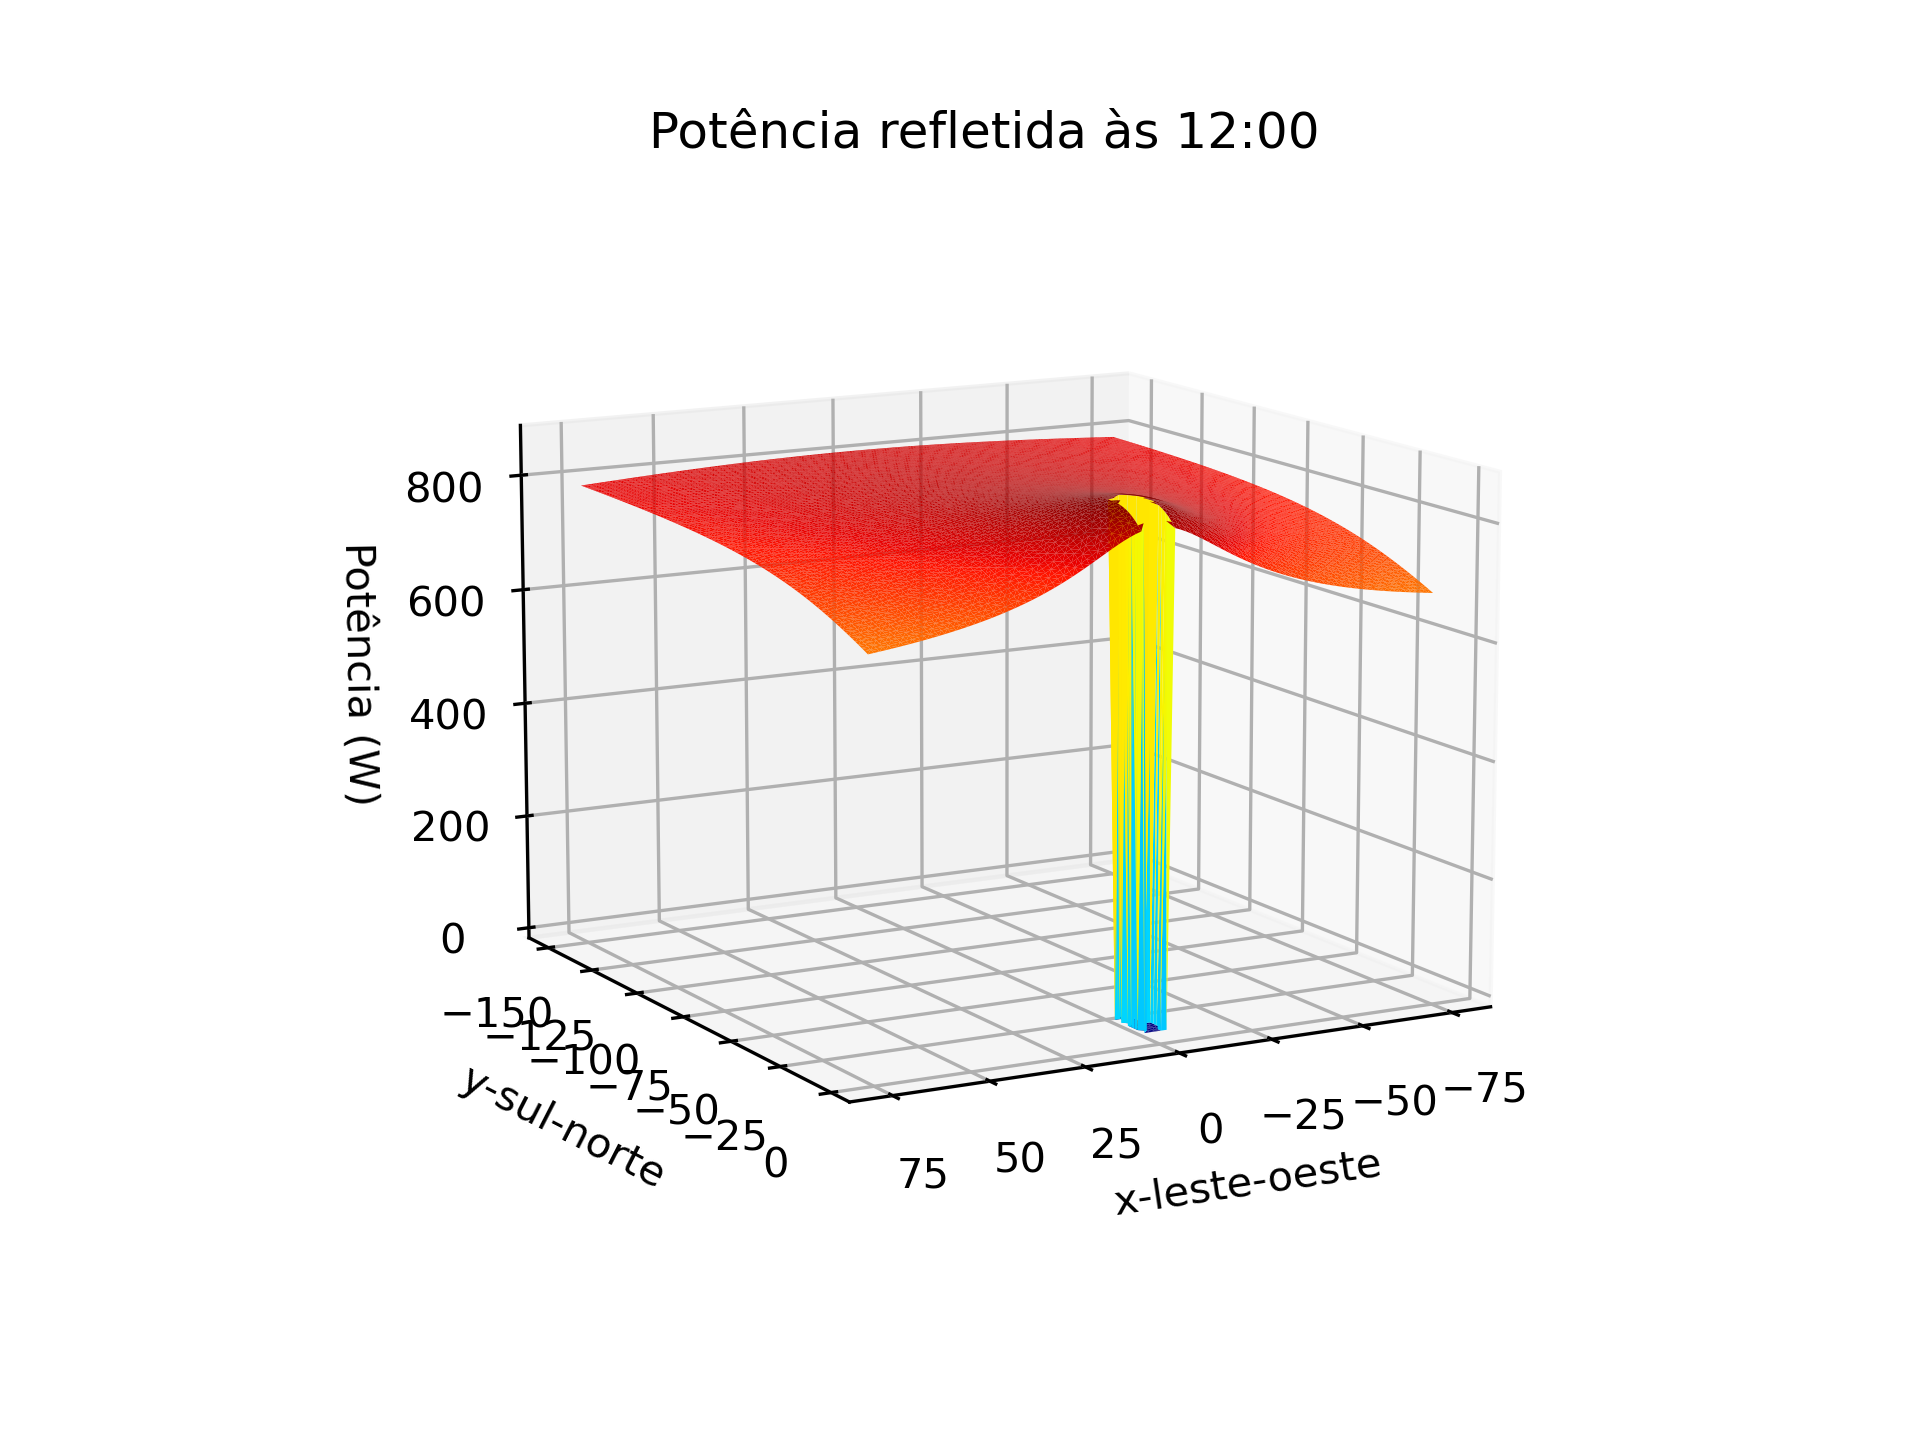
\includegraphics[width=0.8\textwidth]{../../plots/tower_shadow_correction/square_grid_12am.png}
		% \caption{Potência refletida numa torre de $20$m de altura ao meio dia}
		\label{fig:heliost_field_at_12pm}
	\end{figure}
\end{frame}

\begin{frame}%Square grid at 8am
	\begin{figure}[htpb]
		\centering
		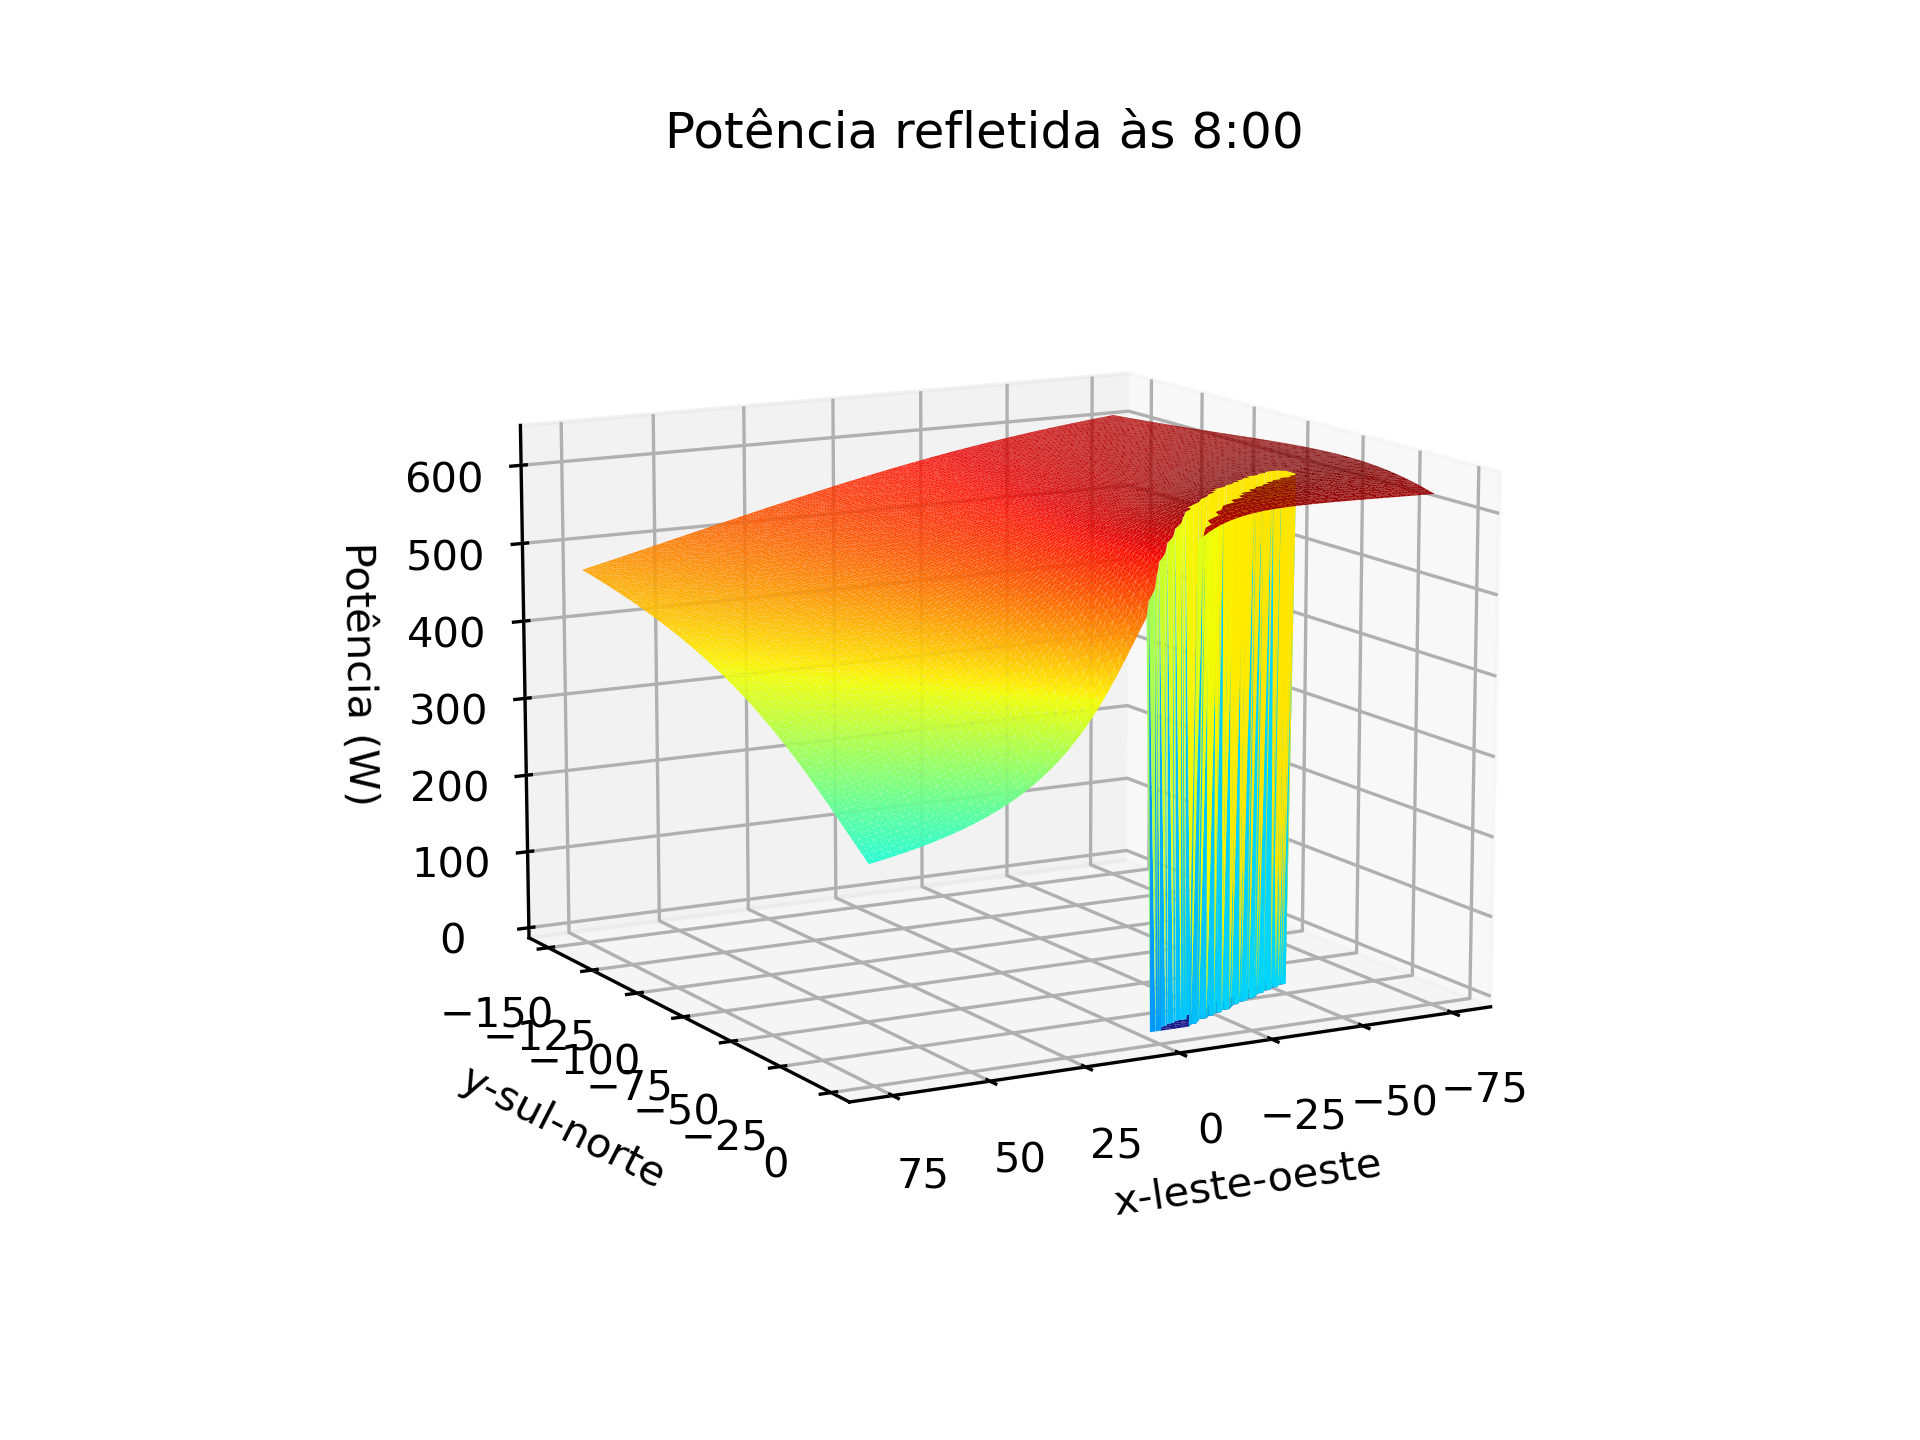
\includegraphics[width=0.8\textwidth]{../../plots/tower_shadow_correction/square_grid_8am.png}
		% \caption{Potência refletida numa torre de $20$m de altura ao meio dia}
		\label{fig:heliost_field_at_8am}
	\end{figure}
\end{frame}

\begin{frame}%Média ao longo do dia
	\begin{figure}[htpb]
		\centering
		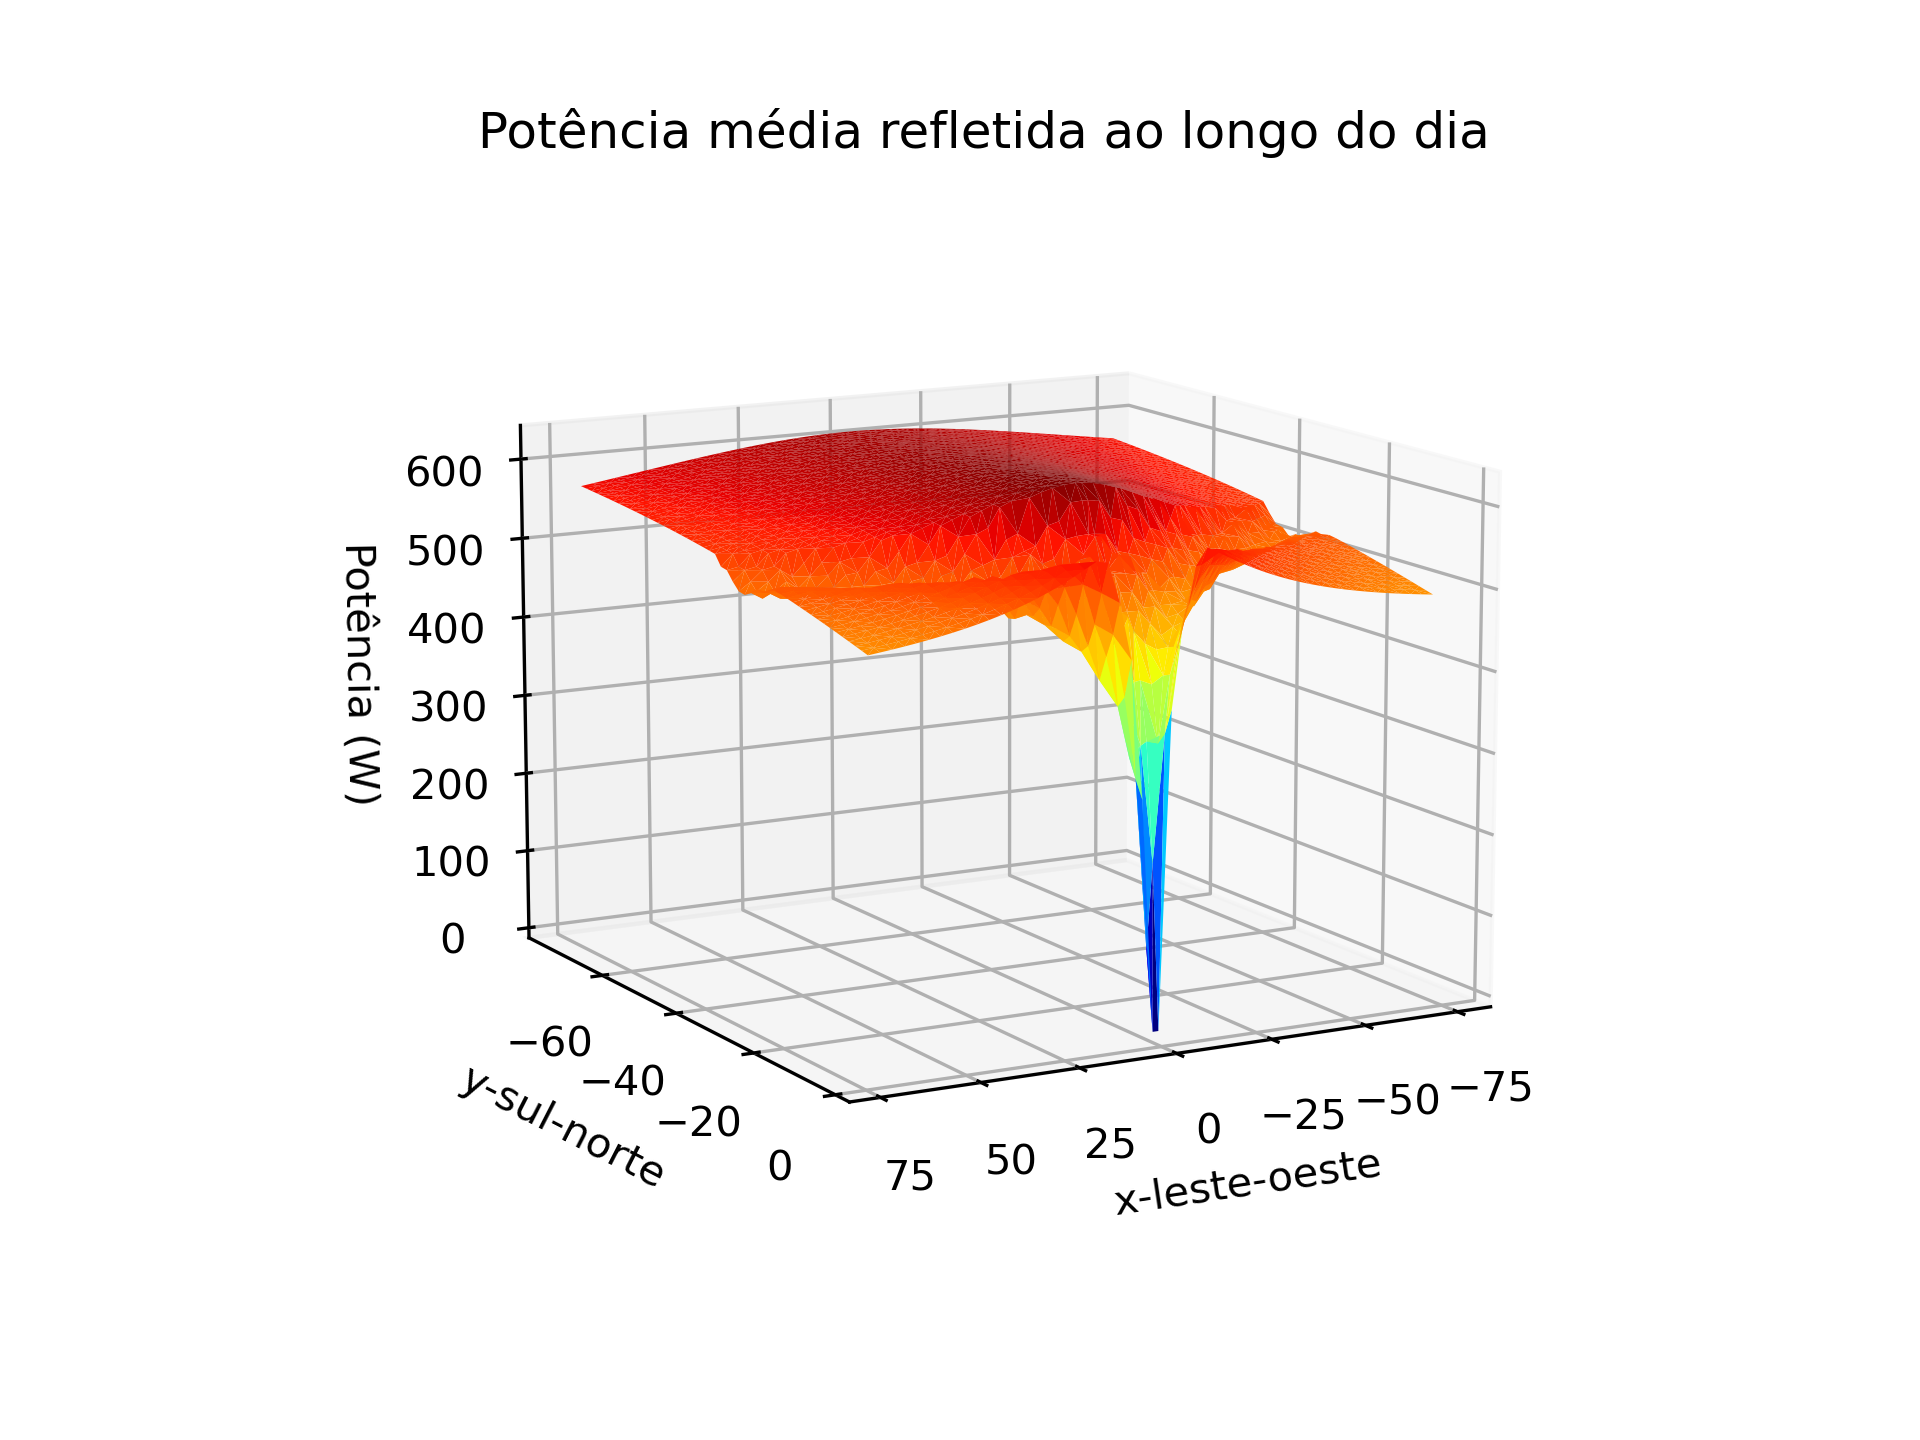
\includegraphics[width=0.8\textwidth]{../../plots/tower_shadow_correction/square_grid_along_day.png}
		% \caption{Potência refletida numa torre de $20$m de altura ao meio dia}
		\label{fig:heliost_field_average}
	\end{figure}
\end{frame}

\end{document}
